\section{Используемые технологии}
\label{sec:technology}

\subsection{Платформа \LB}
\label{sec:technology:logicblox}

В данном подразделе будут рассмотрены основные аспекты разработки приложений на платформе \LB, обзор технологии, архитектуру приложения, а также немного погрузимся в технические аспекты, разберемся в основных отличиях от стандартных приложений.

Первое, с чего следует начать, это с рассмотрения обычной трехслойной архитектуры приложения. При стандартном подходе выделяются Data Store layer (слой базы данных), Business Logic layer (слой бизнес-логики), UI layer (слой представления).

Слой базы данных обеспечивает хранение данных, реализуется в основном средствами систем управления базами данных, подключение к этому компоненту обычно обеспечивается только с уровня сервера приложений. В слое базы данных, как правило, находится не одна база. В большинстве случаев применяются 2 типа: \olap (OnLine Analytical Processing) и \oltp (OnLine Transactional Processing).
\oltp характеризуется большим количеством маленьких транзакций (INSERT, UPDATE, DELETE). Основной упор \oltp систем делается на быструю обработку запросов, управление интегрируемостью данных в мультидоступной среде. Ее эффективность измеряется в количестве транзакций в секунду. В таких базах данные детализированы и схема представляет собой модель сущности (как правило, в 3 нормальной форме).
\olap же характеризуется относительно низкими объемами транзакций. Запросы сами по себе трудоемкие и сложные, часто включают в себя агрегацию. Здесь эффективностью является время ответа на запрос. \olap приложения используются, например, в технологиях Data Mining. Такие базы содержат в себе агрегированные, исторические данные.

Приведем ключевые различия между этими видами в таблице \ref{table:technology:logicblox:oltp_olap_diff}:

\begin{longtable}{|>{\raggedright}m{0.2\textwidth}|>{\raggedright\arraybackslash}m{0.35\textwidth}|>{\raggedright\arraybackslash}m{0.35\textwidth}|}
\caption{Ключевые отличия между \oltp и \olap системами \cite{first_course_in_db}}
\label{table:technology:logicblox:oltp_olap_diff}
\centering
	\hline
	\begin{minipage}{1\linewidth}
		\centering Критерий
	\end{minipage} &
	\begin{minipage}{1\linewidth}
		\centering \oltp
	\end{minipage} &
	\begin{minipage}{1\linewidth}
		\centering \olap
	\end{minipage}
	\endfirsthead
	\caption*{Продолжение таблицы \ref{table:technology:logicblox:oltp_olap_diff}}\\
	\hline
	\centering 1 & \centering 2 & \centering\arraybackslash 3\\
	\hline
	\endhead
	\hline
	\centering 1 & \centering 2 & \centering\arraybackslash 3\\

  \hline Источник даных & Операционные данные, сама база является источником & Консолидированные данные, часто содержит в себе несколько \oltp баз \\
  \hline Цель хранения данных & Контроль и выполнение базовых бизнес-задач & Помощь в планировании, решении проблем, поддержка решений \\
  \hline Что является данными & Представляет собой снимок, или срез, постоянных бизнес-процессов & Многоразмерные содержания различных видов бизнес-активностей \\
  \hline Запросы вставки и обновления & Короткие и быстрые вставки и обновления, инициируемые конечным пользователем & Периодические долго выполняющиеся запросы \\
  \hline Запросы & Как правило стандартизируемые и простые запросы. Возвращают небольшие ответы & Часто сложные запросы с агрегацией \\
  \hline Скорость обработки & Быстрая & Зависит от количества используемых данных; скорость запросов может улучшаться с помощью применения индексов \\
  \hline Требования по памяти & Может быть достаточно небольшая, если исторические данные архивируются & Больше, чем в \oltp, из-за структур для агрегации и исторических данных, требует также больше индексов \\
  \hline Дизайн базы & Большая степень нормализованности со множеством таблиц & Не нормализованная с небольшим количество таблиц, имеют схемы звезды \\
  \hline Резервное копирование & Копируется постоянно. Операционные данные имеют решающее значение для ведения бизнеса, их потеря может привести к значительным денежным затратам и юридической ответственности & Вместо регулярных сохранений некоторые среды могут просто перезагружать \oltp данные в качестве метода восстановления \\
	\hline
\end{longtable}

Как правило, программирование в них идет с помощью \sql, PL/\sql, в \olap возможно применение MDX. При текущих высоких нагрузках также возможно использование \nosql, \hadoop кластера и т.д.

Бизнес-логика обычно работает в сервере приложений (если это веб-приложение). В этом слое применяются такие языки, как \java, \csharp, \python, \scala.
Уровень \ui (слой представления) - веб-приложение с \html и \js. Все эти слои представлены на рисунке \ref{fig:technology:logicblox:three_tier_architecture}.

\begin{figure}
	\centering
	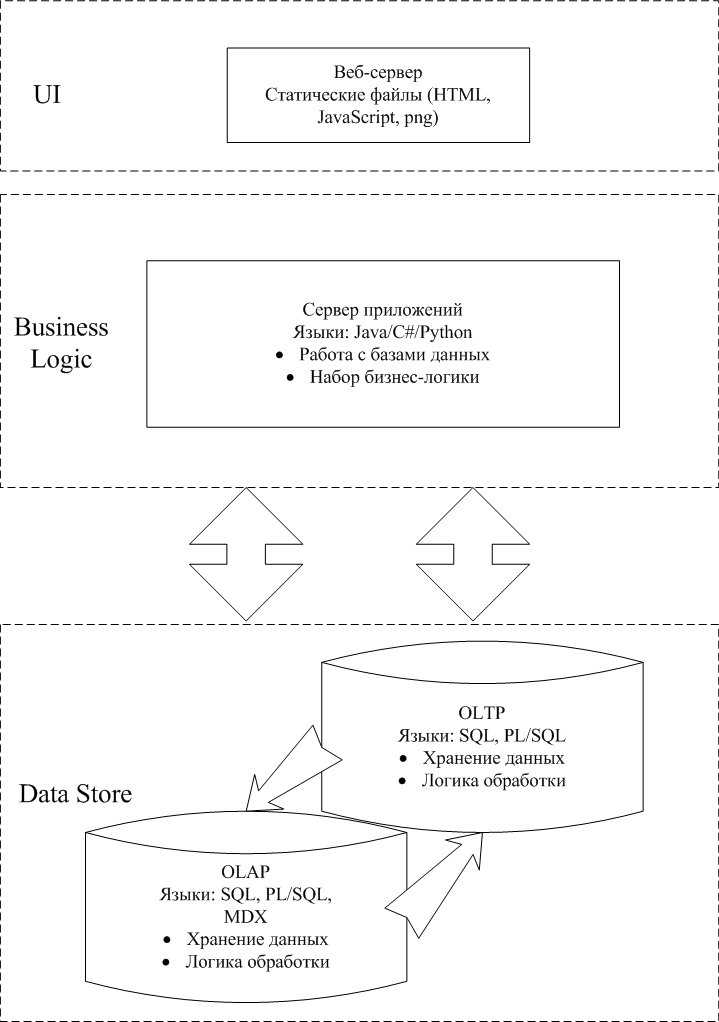
\includegraphics[scale=0.8]{3tier.png}
	\caption{Схема обычного приложения с 3-уровненовой архитектурой}
	\label{fig:technology:logicblox:three_tier_architecture}
\end{figure}

При всем этом существует достаточно большое взаимодействие между сервером приложений и уровнем базы данных. Это не всегда тривиальный код, который преобразует схему базы данных между двумя уровнями. В базе данных все хранится в реляционных таблицах, которые нужно трансформировать в используемые компоненты в сервере приложений, или в объекты. Очевидно, ключевой задачей является минимизация движения этих данных, поскольку в большинстве случаев это не только замедляет работу приложения, но также может быть достаточно дорогой операцией. Зачастую накладывается ограничение на используемую память слоя бизнес-логики, поэтому есть пределы сверху на размер информации.

Более того, если в приложении используются как аналитические запросы, так и транзакционные обновления, необходимо учитывать и взаимодействие между самими \olap и \oltp базами данных. Понятно, что они должны быть синхронизируемы между собой, то есть данные должны быть консистентными. Согласно последним исследованиям на данного рода операции отводится свыше 50\% времени работы баз данных.

В платформе \LB также используется 3-уровневая архитектура, за исключением некоторых ключевых моментов, которые представлены здесь в ином виде. В слое базы данных используется лишь одна база данных вместо нескольких разновидностей. Такая база называется \LB Database, при этом она не построена на основании какой-либо другой (\postgres и т.п.), то есть она разработана «с чистого листа». Благодаря этому она может обрабатывать различные виды нагрузки, которые нужны в рассматриваемой сфере.

Кроме того, здесь используется новый язык \logiql. Основной целью его разработки были легкость выражения хранения данных, а также логики обработки и логики взаимодействия данных. В платформе \LB слой бизнес-логики предельно прост и тонок, поскольку большая часть логики обработки данных заложена именно в самой базе данных. В большинстве приложений вообще нет слоя бизнес-логики как такового - все выполняется в самой базе. В этом случае отпадает необходимость в трудоемком взаимодействии между этими двумя слоями. Кроме того, любое изменения в схеме базы данных отражается лишь в самой базе - нет нужды отслеживать это изменение в другом слое.

Итак, как итог, можно выделить следующие ключевые факторы в платформе \LB:

\begin{itemize}
	\item включает в себя аналитическую, транзакционную обработку данных, содержит математические оптимизационные алгоритмы;
	\item единый декларативный язык программирования \logiql - не стоит учить несколько различных языков;
	\item нет необходимости отслеживания за консистентностью данных между различными базами данных;
	\item может содержать в себе машинное обучение (для компонента прогноза продаж).
\end{itemize}

Схема приложения \LB представлена на рисунке \ref{fig:technology:logicblox:lb_architecture}.

\begin{figure}
	\centering
	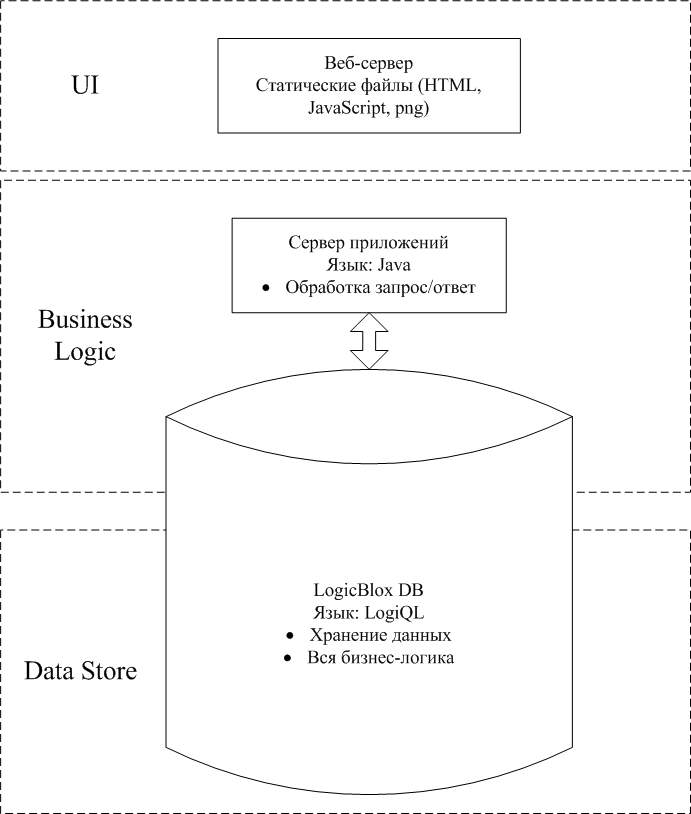
\includegraphics[scale=1]{lb_architecture.png}
	\caption{Схема приложения \LB с 3-уровневой архитектурой \cite{lb_platform}}
	\label{fig:technology:logicblox:lb_architecture}
\end{figure}

Посмотрим на состав самой базы. В ней находится 3 сегмента \cite{lb_db_overview}:

\begin{enumerate}
	\item Определение схемы, как и в других базах данных, с полями, колонками, ограничениями. Пример предикатов:
	\begin{lstlisting}[language=Prolog]
	sales_u(product, store, day, unit) ->
		string(product),
		string(store),
		datetime(day),
		int(unit).

	returns_u(product, store, day, units) ->
		string(product),
		string(store),
		datetime(day),
		int(units).
	\end{lstlisting}
	\item Бизнес-правила:
	\begin{lstlisting}[language=Prolog]
	netsales_u(product, store, day, net) <-
	  sales_u(product, store, day, sls),
	  returns_u(product, store, day, returns),
	  net = sls - returns.
	\end{lstlisting}
	\item Конфигурация сервисов, которые сервер приложений будет использовать для тех или иных целей \cite{query_language_for_smart_db}.
\end{enumerate}
